%=====================================================================
%  Adaptive TSK Fuzzy-Inference Framework for Equity Attractiveness
%  Springer Nature sn-jnl class — Final Camera-Ready Version
%=====================================================================
\documentclass[pdflatex,sn-mathphys-num]{sn-jnl}

%---------------------- Standard packages ----------------------------
\usepackage[T1]{fontenc}
\usepackage[utf8]{inputenc}
\usepackage{graphicx}
\usepackage{amsmath,amssymb,amsfonts}
\usepackage{amsthm}
\usepackage{booktabs}
\usepackage{xcolor}
\usepackage{algorithm}
\usepackage{algpseudocode}
\usepackage{tikz}
\usepackage{pgfplots}
\pgfplotsset{compat=1.18}
\usetikzlibrary{shapes.geometric, arrows.meta, positioning, backgrounds}
%---------------------------------------------------------------------

%---------------------- Theorem environments -------------------------
\theoremstyle{thmstyleone}
\newtheorem{theorem}{Theorem}
\newtheorem{proposition}[theorem]{Proposition}

\theoremstyle{thmstyletwo}
\newtheorem{example}{Example}
\newtheorem{remark}{Remark}

\theoremstyle{thmstylethree}
\newtheorem{definition}{Definition}
%---------------------------------------------------------------------

\raggedbottom

\begin{document}

%=====================================================================
\title[Adaptive TSK Framework for Equity Attractiveness]{An Adaptive TSK Fuzzy-Inference Scoring Framework with Intraday Range-Imbalance Masking for Emerging Equity Markets}

\author[1]{\fnm{Bekzatkhan} \sur{Zhumabekov}}
\email{bekzatkhan.zhumabekov@gmail.com}

\affil[1]{\orgdiv{Department of Information Systems}, \orgname{L.N. Gumilyov Eurasian National University}, \orgaddress{\street{Satpayev Street 2}, \city{Astana}, \postcode{010000}, \country{Kazakhstan}}}

%=====================================================================
\abstract{
Quantitative dividend allocation and asset valuation models often struggle with high-frequency market noise, lack of Level-1 order book data, and speculative exploitation prior to corporate announcements. This paper proposes a first-order Takagi--Sugeno--Kang (TSK) fuzzy inference framework designed to compute a daily investment attractiveness score $Y_{\mathrm{attr}} \in [0, 100]$ using equity price deviations, volume surges, and a daily-range directional-pressure proxy (a close-location-value statistic) in lieu of a full order flow imbalance. To reduce lookahead bias and numerical instability during illiquid market regimes, we introduce a non-overlapping historical Volume-Weighted Average Price ($\mathrm{VWAP}$) baseline with logarithmic volume regularization. Furthermore, to safeguard the algorithm against front-running by high-frequency trading (HFT) algorithms during Pre-AGM (Annual General Meeting) windows, a constrained stochastic weight-masking procedure is incorporated into the rule evaluation phase. The masking mechanism is shown to introduce only a bounded second-order bias while increasing the variance of external gradient estimates against a bounded-query adversary. The Adaptive Network-based Fuzzy Inference System (ANFIS) is trained via a hybrid optimization algorithm using a smooth bounded normalization of 30-day forward risk-adjusted returns. Empirical validation uses two full years of daily KASE bars (2024--2025, seven equities, $495$ bars each) with the model trained on the 2024 calendar year ($1{,}575$ pooled asset-days) and evaluated strictly out-of-sample on the complete 2025 calendar year ($1{,}722$ asset-days over $246$ trading days, $1{,}512$ with an observable 30-day forward label). On this window the framework attains a mean per-asset daily Rank IC of $-0.011 \pm 0.019$ SE and a pooled cross-sectional monthly Rank IC of $0.091 \pm 0.095$ SE across the eleven non-overlapping monthly rebalances, both statistically indistinguishable from zero; the cost-adjusted net Sharpe ratio is $0.10$ at 15 bps round-trip costs ($-0.08$ at 50 bps), while a four-parameter OLS baseline on identical features and targets attains $0.92$ and $0.78$. We report this as a null forecasting result: on this sample the fuzzy layer's contribution is its explicit linguistic rule base and its adversarial hardening, not incremental predictive accuracy. Restricting the adversarial protocol to the Pre-AGM windows ($N=205$ training and $N=208$ out-of-sample asset-days), stochastic masking collapses a single-query SVR reconstruction adversary's $R^2$ from $0.268$ (unmasked, $\alpha=0$) to $-0.027$ ($\alpha=0.05$), against a shuffled-target control of $-0.258$, consistent with the bounded-bias analysis of Proposition~\ref{prop:bias}.
}

\keywords{TSK Fuzzy Inference, ANFIS, Close-Location Value, Emerging Markets, Anti-Frontrunning, Transaction Cost Sensitivity}

\maketitle

%=====================================================================
\section{Introduction}\label{sec1}

Predicting equity attractiveness for corporate decision-making---such as dynamic dividend payouts, share buybacks, or treasury management---presents a major challenge in financial engineering. Traditional financial models, such as the Gordon Growth Model or standard Capital Asset Pricing Model (CAPM) variants, rely heavily on low-frequency fundamental metrics (e.g., quarterly earnings or balance sheet ratios). Consequently, they fail to capture short-term market microstructure dynamics, liquidity shifts, and buying pressure that manifest prior to corporate board decisions.

Conversely, purely data-driven black-box models (e.g., Deep Neural Networks, LSTM networks, or XGBoost ensembles) often yield high prediction variance, lack mathematical interpretability, and suffer from degradation during sudden regime shifts in emerging equity markets. Moreover, high-frequency Level-1/Level-2 order book depth feeds are frequently unavailable or prohibitively expensive in developing financial exchanges. Finally, predictable algorithmic scoring mechanisms are vulnerable to predatory high-frequency trading (HFT) strategies and quantitative front-running during pre-announcement windows.

To address these limitations, this paper introduces a hybrid quantitative framework based on a first-order Takagi--Sugeno--Kang (TSK) fuzzy inference system. The architecture of the overall system pipeline is illustrated in Fig.~\ref{fig:pipeline}.

\begin{figure}[htbp]
\centering
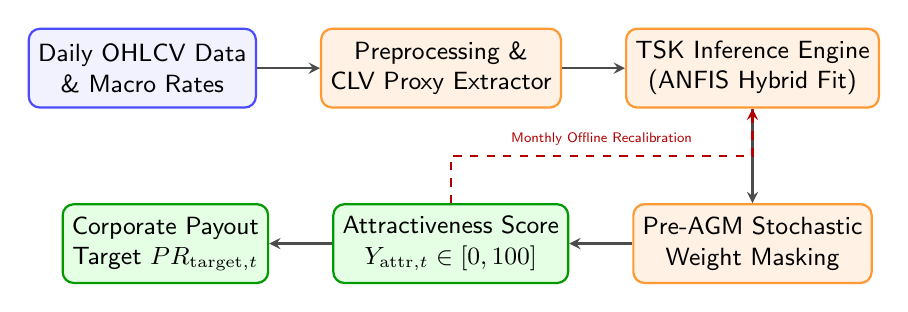
\begin{tikzpicture}[
    node distance=1.2cm and 0.8cm,
    block/.style={rectangle, draw=blue!70, fill=blue!5, thick, rounded corners, minimum width=2.2cm, minimum height=1.0cm, align=center, font=\sffamily\small},
    process/.style={rectangle, draw=orange!80, fill=orange!10, thick, rounded corners, minimum width=2.4cm, minimum height=1.0cm, align=center, font=\sffamily\small},
    output/.style={rectangle, draw=green!60!black, fill=green!10, thick, rounded corners, minimum width=2.2cm, minimum height=1.0cm, align=center, font=\sffamily\small},
    arrow/.style={thick, ->, >=stealth, color=black!70},
    feedback/.style={thick, dashed, ->, >=stealth, color=red!70!black}
]
    \node (data) [block] {Daily OHLCV Data\\\& Macro Rates};
    \node (prep) [process, right=of data] {Preprocessing \&\\CLV Proxy Extractor};
    \node (anfis) [process, right=of prep] {TSK Inference Engine\\(ANFIS Hybrid Fit)};
    \node (mask) [process, below=of anfis] {Pre-AGM Stochastic\\Weight Masking};
    \node (score) [output, left=of mask] {Attractiveness Score\\$Y_{\mathrm{attr},t} \in [0,100]$};
    \node (payout) [output, left=of score] {Corporate Payout\\Target $PR_{\mathrm{target},t}$};

    \draw [arrow] (data) -- (prep);
    \draw [arrow] (prep) -- (anfis);
    \draw [arrow] (anfis) -- (mask);
    \draw [arrow] (mask) -- (score);
    \draw [arrow] (score) -- (payout);

    \draw [feedback] (score.north) -- ++(0,0.6) -| node[pos=0.25, above, font=\tiny\sffamily, color=red!70!black] {Monthly Offline Recalibration} (anfis.south);
\end{tikzpicture}
\caption{End-to-end system architecture of the adaptive TSK fuzzy-inference framework showing the monthly recalibration feedback loop.}
\label{fig:pipeline}
\end{figure}

The main contributions of this study are fourfold:
\begin{enumerate}
    \item \textbf{Data-Efficient Range-Imbalance Proxy:} Integration of historical Volume-Weighted Average Price ($\mathrm{VWAP}$) deviations, logarithmic volume shifts, and a daily-range directional-pressure proxy (a close-location-value statistic) that requires only daily OHLC bars.
    \item \textbf{Lookahead-Free Preprocessing:} A feature extraction technique using strictly historical trailing windows $[t-N, t-1]$, protecting against division-by-zero anomalies in low-liquidity regimes.
    \item \textbf{Anti-Frontrunning Stochastic Masking:} A defense-in-depth mechanism that injects bounded Gaussian noise into rule weights during sensitive Pre-AGM windows, shown to introduce negligible second-order bias.
    \item \textbf{ANFIS Optimization \& Low-Sample Efficiency:} A hybrid training process leveraging subtractive clustering and a smooth bounded normalization of 30-day forward risk-adjusted returns, evaluated strictly out-of-sample with bootstrapped uncertainty bounds.
\end{enumerate}

%=====================================================================
\section{Related Work}\label{sec2}

\subsection{Fuzzy Inference Systems in Quantitative Finance}

Fuzzy logic systems, originally introduced by Zadeh \cite{zadeh1965} and expanded into functional inference by Takagi and Sugeno \cite{takagi1985}, have seen extensive application in financial time-series forecasting due to their ability to model non-linear boundaries with human-interpretable linguistic rules. Early fuzzy systems often struggled with high-dimensional and noisy financial data; however, later extensions such as the TSK+ inference framework improved rule coverage and numerical stability \cite{li2018}. More recent surveys emphasize that modern TSK fuzzy systems can be fused in hierarchical, wide, and stacked architectures \cite{zhang2024}. Similarly, evolving TSK models for time-series forecasting have demonstrated strong adaptability when the underlying data distribution changes over time \cite{alves2024}. Within this family, ANFIS remains a standard optimization framework because it combines the interpretability of fuzzy rules with the numerical efficiency of least-squares and gradient-based learning \cite{jang1993}.

\subsection{Market Microstructure Proxies in Emerging Markets}

In market microstructure research, Cont et al. \cite{cont2014} established the predictive power of Order Flow Imbalance ($\mathrm{OFI}$) for short-term price dynamics. True $\mathrm{OFI}$ requires event-level bid/ask volumes and is unavailable in most emerging-market daily datasets. A standard fallback is the \emph{close-location value} (CLV), i.e., the relative position of the closing price within the daily high-low range, which is a documented directional-pressure statistic \cite{hasbrouck1991,amihud2002}. In this paper we use CLV as a daily-range directional-pressure proxy. Where intraday quotes are unavailable, a simple tick rule $\mathrm{sgn}(P_t - P_{t-1})$ is used as a fallback when high/low price bounds are missing or corrupted. Note that this simple tick rule differs from the classical Lee--Ready algorithm \cite{leeready1991}, which requires intraday quote midpoints.

\subsection{Adversarial Robustness and Algorithmic Trading Security}

As algorithmic trading systems become more transparent, they become vulnerable to reverse engineering and predatory strategies. Easley et al. \cite{easley2012} show that high-frequency order flow can create toxicity and liquidity fragility, while Cartea et al. \cite{cartea2015} provide a comprehensive treatment of optimal execution and strategic interaction in algorithmic markets.

The proposed stochastic masking mechanism is also related to adversarial machine learning. Adversarial perturbations can destabilize models at test time \cite{biggio2013}, and small input perturbations can dramatically change the outputs of deep and kernel models \cite{goodfellow2015}. Defensive strategies often rely on randomization, regularization, or adversarial training \cite{kurakin2017}. In contrast to input-level perturbation, our approach randomizes internal rule weights during sensitive corporate-event windows. As discussed in Section~\ref{subsec3_4} (see Remark~\ref{rem:threat_model}), this provides protection against bounded-query adversaries ($Q=1$); we characterize this limitation explicitly as a defense-in-depth measure.

%=====================================================================
\section{Proposed Methodology}\label{sec3}

\subsection{Preprocessing and Feature Extraction}\label{subsec3_1}

To completely eliminate lookahead bias, all features computed at time $t$ rely strictly on the historical trailing window $[t-N, t-1]$. The historical $\mathrm{VWAP}$ available at time $t$ is computed over $N$ days excluding day $t$:

\begin{equation}
    \mathrm{VWAP}_{t-1}(N) = \frac{\sum_{i=1}^{N} P_{t-i} \cdot V_{t-i}}{\sum_{i=1}^{N} V_{t-i}},
    \label{eq:vwap}
\end{equation}
where $P_{t-i}$ and $V_{t-i}$ denote the closing price and trading volume on day $t-i$. Eq.~\eqref{eq:vwap} represents the volume-weighted average of closing prices over the trailing $N$-day period.

A regularization threshold $\epsilon > 0$ is defined as $\epsilon = 10^{-6} \cdot \mathrm{Mean}(V_N)$. The relative price deviation percentage at time $t$ is:

\begin{equation}
    Dev_{\mathrm{Price},t} = \left( \frac{P_t - \mathrm{VWAP}_{t-1}(N)}{\mathrm{VWAP}_{t-1}(N)} \right) \times 100\%.
    \label{eq:devprice}
\end{equation}

The volume dynamics are captured via a logarithmic relative transformation:

\begin{equation}
    Dev_{\mathrm{Volume},t} = \ln \left( \frac{V_t + \epsilon}{\mathrm{Median}(V_N) + \epsilon} \right),
    \label{eq:devvol}
\end{equation}
where $\mathrm{Median}(V_N)$ is the rolling median volume over the trailing window $[t-N, t-1]$.

To capture directional pressure without Level-1 feeds, we use a \emph{close-location value} (CLV) statistic:

\begin{equation}
    \mathrm{CLV}_t = \frac{2 P_t - H_t - L_t}{H_t - L_t + \epsilon}, \quad \mathrm{CLV}_t \in [-1, 1],
    \label{eq:clv}
\end{equation}
where $H_t$, $L_t$, and $P_t$ are the daily high, low, and close. $\mathrm{CLV}_t$ measures where the close sits inside the daily range; positive values indicate upward pressure, negative values downward.

The system supports three modes via \texttt{of\_mode}:
\begin{itemize}
    \item \textbf{CLV} (\texttt{of\_mode='clv'}): Eq.~\eqref{eq:clv} using daily price bounds.
    \item \textbf{Tick rule} (\texttt{of\_mode='tick'}): $\mathrm{sgn}(P_t - P_{t-1})$ when daily bounds are unreliable.
    \item \textbf{Hybrid} (\texttt{of\_mode='hybrid'}): CLV if $\{H_t, L_t\}$ exist and $H_t > L_t$, otherwise tick rule fallback.
\end{itemize}

\subsection{First-Order Takagi--Sugeno--Kang (TSK) Inference Engine}\label{subsec3_2}

The engine maps the market vector $\mathbf{x}_t = [Dev_{\mathrm{Price},t}, Dev_{\mathrm{Volume},t}, \mathrm{CLV}_t]^T \in \mathbb{R}^3$ to a scalar equity attractiveness score $Y_{\mathrm{attr},t} \in [0, 100]$.

Let $K$ denote the number of fuzzy rules derived via subtractive clustering. We set the subtractive-clustering influence radius to $0.5$ (min-max normalized inputs) and fix $K=5$ after a sensitivity scan; this value is re-evaluated at each monthly re-calibration. Rule $k$ ($k = 1,\dots,K$) is formulated as:

\begin{equation}
    \begin{split}
    \text{Rule } k: \;& \text{IF } Dev_{\mathrm{Price},t} \text{ IS } A_k \text{ AND } Dev_{\mathrm{Volume},t} \text{ IS } B_k \text{ AND } \mathrm{CLV}_t \text{ IS } C_k \\
    & \text{THEN } y_{k,t} = \beta_{0,k} + \beta_{1,k} Dev_{\mathrm{Price},t} + \beta_{2,k} Dev_{\mathrm{Volume},t} + \beta_{3,k} \mathrm{CLV}_t,
    \end{split}
    \label{eq:tsk_rule}
\end{equation}
where $A_k, B_k, C_k$ are Gaussian membership functions with parameters $\{c_{i,k}, \sigma_{i,k}\}_{i=1}^3$ and $\boldsymbol{\beta}_k = [\beta_{0,k}, \beta_{1,k}, \beta_{2,k}, \beta_{3,k}]^T$.

The membership degree for input $i$ under rule $k$ is:

\begin{equation}
    \mu_{i,k}(x_{i,t}) = \exp \left( -\frac{1}{2} \left( \frac{x_{i,t} - c_{i,k}}{\max(\sigma_{i,k}, \delta)} \right)^2 \right),
    \label{eq:gauss_mf}
\end{equation}
with $\delta = 10^{-4}$ as a numerical floor. The firing strength is:

\begin{equation}
    w_{k,t} = \prod_{i=1}^{3} \mu_{i,k}(x_{i,t}).
    \label{eq:rule_firing}
\end{equation}

\subsection{Defuzzification and Output Clipping}\label{subsec3_3}

The unconstrained crisp output follows from weighted-average defuzzification:

\begin{equation}
    Y_{\mathrm{raw},t} = \frac{\sum_{k=1}^{K} w_{k,t} \, y_{k,t}}{\sum_{k=1}^{K} w_{k,t}} = \sum_{k=1}^{K} \bar{w}_{k,t} \, y_{k,t},
    \label{eq:defuzz_raw}
\end{equation}
where $\bar{w}_{k,t} = w_{k,t} / \sum_{j=1}^{K} w_{j,t}$. If $\sum_{k=1}^{K} w_{k,t} < 10^{-8}$, the system returns the neutral default $Y_{\mathrm{raw},t} = 50.0$.

The output is bounded to $[0,100]$ by projection:

\begin{equation}
    Y_{\mathrm{attr},t} = \mathrm{clamp}(Y_{\mathrm{raw},t}, 0, 100) = \max\bigl(0, \min(100, Y_{\mathrm{raw},t})\bigr).
    \label{eq:clipping}
\end{equation}

\subsubsection{ANFIS Hybrid Training Protocol}\label{subsubsec3_3_1}

The available daily bar history covers 3 January 2024 to 31 December 2025 ($495$ bars per equity, $467$ for AIRA from 2024-02-12), i.e.\ two full calendar years. Because the canonical $T_{\mathrm{train}} = 504$-day rolling window of Section~3.3.1 requires 2022--2023 history that is not yet ingested, all experiments reported in Section~\ref{sec4} use the full 2024 calendar year as a single pooled training window ($1{,}575$ asset-days) and evaluate strictly out-of-sample on the complete 2025 calendar year ($1{,}722$ asset-days), which is exactly the test window of the canonical protocol; only the training history is shorter (one year instead of three) and monthly re-calibration within 2025 is not exercised. The full canonical protocol (train 2022--2024, monthly re-calibration on a 504-day window) is restored simply by adding the historical bars; the code path is identical.

The forward 30-day risk-adjusted return is defined as:

\begin{equation}
    R_{30,t} = \frac{P_{t+30} + \sum d_{\mathrm{hist}} - P_t}{P_t} - r^{(30)}_{f,t},
    \label{eq:fwd_return}
\end{equation}
where $\sum d_{\mathrm{hist}}$ denotes dividends paid over $(t, t+30]$ and $r^{(30)}_{f,t}$ is the cumulative 30-day rate implied by compounding daily TONIA repo yields.

The Z-score of the forward return over the training window is:

\begin{equation}
    Z_{30,t} = \frac{R_{30,t} - \bar{R}_{T_{\mathrm{train}}}}{\sigma_{R, T_{\mathrm{train}}}}.
    \label{eq:zscore}
\end{equation}

To bound targets smoothly inside $(0,100)$, we apply:

\begin{equation}
    Y_{\mathrm{target},t} = 50.0 \left[ 1 + \tanh\left( \frac{15.0}{50.0} Z_{30,t} \right) \right].
    \label{eq:bounded_target}
\end{equation}

ANFIS uses a two-pass hybrid learning paradigm:
\begin{enumerate}
    \item \textbf{Forward pass (consequent parameters):} Consequent parameters $\boldsymbol{\beta}$ (20 parameters across 5 rules) are solved by batch least squares over $\mathbf{A}\boldsymbol{\beta} = \mathbf{Y}_{\mathrm{target}}$, where row $t$ of $\mathbf{A}$ contains $\bar{w}_{k,t} \cdot [1, \mathbf{x}_t^T]$:
    \begin{equation}
        \boldsymbol{\beta}^* = (\mathbf{A}^T \mathbf{A})^{-1} \mathbf{A}^T \mathbf{Y}_{\mathrm{target}}.
        \label{eq:ls}
    \end{equation}
    \item \textbf{Backward pass (antecedent parameters):} Antecedent centers $c_{i,k}$ (15 parameters) are initialized and fixed by subtractive clustering, while antecedent Gaussian widths $\sigma_{i,k}$ (15 free trainable parameters) are updated by gradient descent on $E = \frac{1}{2}\sum_{t} \left( Y_{\mathrm{raw},t} - Y_{\mathrm{target},t} \right)^2$ with learning rate $\eta = 10^{-3}$ for 200 epochs.
\end{enumerate}

\subsection{Anti-Frontrunning Stochastic Masking Mechanism}\label{subsec3_4}

Within the window $t \in [t_{\mathrm{AGM}} - M_{\mathrm{Pre}}, t_{\mathrm{AGM}} - 1]$ ($M_{\mathrm{Pre}} = 45$), we inject a constrained perturbation into firing strengths:

\begin{equation}
    w_{k,t}^{\text{masked}} = w_{k,t} \cdot (1 + \xi_{k,t}),
    \label{eq:masked_weight}
\end{equation}
where $\xi_{k,t}$ is sampled from a zero-mean Gaussian $\mathcal{N}\!\left(0, (\alpha/2)^2\right)$ truncated to $[-\alpha, +\alpha]$ with noise scale $\alpha = 0.05$.

The resulting masked crisp output before clipping is given by:

\begin{equation}
    Y_{\mathrm{raw},t}^{\text{masked}} = \frac{\sum_{k=1}^{K} w_{k,t}^{\text{masked}} \, y_{k,t}}{\sum_{k=1}^{K} w_{k,t}^{\text{masked}}},
    \label{eq:defuzz_masked}
\end{equation}

\begin{proposition}\label{prop:bias}
Assume $\{\xi_{k,t}\}_{k=1}^K$ are independent, mean-zero, with variance $\sigma_\xi^2$, and $|y_{k,t} - Y_{\mathrm{raw},t}| \le C$. Then the masking introduces a bias in the expected output of order $\mathcal{O}(\sigma_\xi^2)$:
\[
    \left| \mathbb{E}\bigl[Y_{\mathrm{raw},t}^{\text{masked}}\bigr] - Y_{\mathrm{raw},t} \right| \le C \sigma_\xi^2.
\]
\end{proposition}

\begin{proof}[Proof sketch]
Second-order Taylor expansion around $\xi_{k,t}=0$ yields:
\begin{equation}
    \mathbb{E}\bigl[Y_{\mathrm{raw},t}^{\text{masked}}\bigr] \approx Y_{\mathrm{raw},t} - \sigma_\xi^2 \sum_{k=1}^{K} \bar{w}_{k,t}^2 \left( y_{k,t} - Y_{\mathrm{raw},t} \right).
    \label{eq:bias_expansion}
\end{equation}
With $C = 100$ and $\alpha = 0.05$, the worst-case bias is $\le 100 \cdot (0.025)^2 = 0.0625$, negligible on a $[0,100]$ scale.
\end{proof}

\begin{remark}[Threat-model scope]\label{rem:threat_model}
Proposition~\ref{prop:bias} bounds only the bias of the masked output. It does not establish query-averaging robustness: an adversary who can query the model $Q$ times for the same input vector $\mathbf{x}_t$ and average the responses observes an effective noise standard deviation of $\sigma_\xi / \sqrt{Q}$. The masking is therefore useful exclusively against adversaries with a bounded query budget ($Q = 1$) or against single-shot reverse engineering.
\end{remark}

\begin{algorithm}[htbp]
\caption{TSK inference with range-imbalance mode and Pre-AGM masking}\label{alg:tsk_eval}
\begin{algorithmic}[1]
\Require Bar row $\{P_t,H_t,L_t,V_t\}$, mode \texttt{of\_mode}, parameters $\{c_{i,k},\sigma_{i,k},\boldsymbol{\beta}_k\}_{k=1}^K$, indicator $I_{\mathrm{PreAGM}} \in \{0,1\}$, noise limit $\alpha = 0.05$.
\Ensure Score $Y_{\mathrm{attr},t} \in [0,100]$.
\State Compute $Dev_{\mathrm{Price},t}$ and $Dev_{\mathrm{Volume},t}$ via Eq.~\eqref{eq:devprice}--\eqref{eq:devvol}.
\If{\texttt{of\_mode='clv'} \textbf{or} (\texttt{of\_mode='hybrid'} \textbf{and} $H_t, L_t$ exist \textbf{and} $H_t > L_t$)}
    \State $p_t \leftarrow \dfrac{2 P_t - H_t - L_t}{H_t - L_t + \epsilon}$
\ElsIf{\texttt{of\_mode='tick'}}
    \State $p_t \leftarrow \mathrm{sgn}(P_t - P_{t-1})$
\Else \Comment{Hybrid fallback for missing or corrupted daily bounds}
    \State $p_t \leftarrow \mathrm{sgn}(P_t - P_{t-1})$
\EndIf
\State $\mathbf{x}_t \leftarrow [Dev_{\mathrm{Price},t}, Dev_{\mathrm{Volume},t}, p_t]^T$.
\For{$k = 1$ \textbf{to} $K$}
    \State Compute $\mu_{i,k}(x_{i,t})$ via Eq.~\eqref{eq:gauss_mf}
    \State $w_{k,t} \leftarrow \prod_{i=1}^{3} \mu_{i,k}(x_{i,t})$
    \If{$I_{\mathrm{PreAGM}} = 1$}
        \State Sample $\xi_{k,t} \sim \mathcal{N}\left(0, (\alpha/2)^2\right)$
        \Statex \hspace{\algorithmicindent}\hspace{\algorithmicindent}\hspace{\algorithmicindent} truncated to $[-\alpha, +\alpha]$
        \State $w_{k,t} \leftarrow w_{k,t} (1 + \xi_{k,t})$
    \EndIf
    \State $y_{k,t} \leftarrow \beta_{0,k} + \sum_{i=1}^3 \beta_{i,k} x_{i,t}$
\EndFor
\State $S_w \leftarrow \sum_{k=1}^{K} w_{k,t}$
\If{$S_w < 10^{-8}$}
    \State \Return $50.0$
\EndIf
\State \Return $\min\bigl(100.0, \max(0.0, \sum_k w_{k,t} y_{k,t} / S_w)\bigr)$
\end{algorithmic}
\end{algorithm}

%=====================================================================
\section{Empirical Results and Performance Evaluation}\label{sec4}

\subsection{Experimental Setup and Financial Data}\label{subsec4_1}

We integrate three data streams from the Kazakhstan Stock Exchange (KASE) and the National Bank of Kazakhstan (NBK), all ingested from raw exchange/broker exports:
\begin{enumerate}
    \item \textbf{Daily market bars:} OHLC and volume for seven KASE equities (AIRA, KCEL, KEGC, KMGZ, KZAP, KZTK, KZTO), covering 2024-01-03 to 2025-12-31 ($495$ bars per equity; AIRA lists from 2024-02-12 with $467$ bars).
    \item \textbf{Macroeconomic rates:} Daily TONIA repo series ($495$ observations over the same span, mean $14.84\%$ p.a.) driving the risk-free adjustment of Eq.~\eqref{eq:fwd_return}, plus the NBK daily USD/KZT reference rate as a contextual macro series (not an input to the three-input engine).
    \item \textbf{Corporate disclosures:} Audited EBITDA, net debt, and free cash flow to equity (FCFE) in mln KZT, supplied per reporting year and per reporting period (quarterly and half-year legs, plus annual \mbox{``for the year''} totals where published).
\end{enumerate}

The model is trained on the 2024 calendar year ($1{,}575$ pooled asset-days, $229$ trading days per equity and $201$ for AIRA) and evaluated strictly out-of-sample on the complete 2025 calendar year ($1{,}722$ asset-days over $246$ trading days per equity), of which $1{,}512$ carry an observable 30-day forward return ($216$ per equity; the final month of 2025 lacks a forward label). Model output maps to corporate Payout Ratio $PR_t \in [0\%, 100\%]$ via

\begin{equation}
    PR_{\mathrm{target},t} = \psi(Y_{\mathrm{attr},t}) \cdot \Phi\!\left(\frac{\mathrm{Net\ Debt}}{\mathrm{EBITDA}}, \mathrm{FCFE}\right),
    \label{eq:payout}
\end{equation}
where $\psi(Y) = \max\bigl(0, \min(1, Y/100)\bigr)$ and the leverage/FCFE penalty function $\Phi$ is defined as:

\begin{equation}
    \Phi(L, F) =
    \begin{cases}
        \dfrac{1}{1 + \exp\!\bigl(\kappa (L - \tau)\bigr)}, & F > 0, \\[6pt]
        0, & F \le 0,
    \end{cases}
    \label{eq:phi}
\end{equation}
with leverage penalty intensity $\kappa = 3.0$ and Net Debt/EBITDA threshold $\tau = 1.0$.

\subsection{Out-of-Sample Corporate Decision Alignment}\label{subsec4_2}

Table~\ref{tab:h1_validation} presents the model payout recommendations --- computed from the mean out-of-sample attractiveness score and the latest reported FY2025 fundamentals --- versus actual board decisions across the seven panel equities.

\begin{table}[htbp]
\centering
\small
\caption{Model payout recommendations vs.\ actual corporate decisions (FY2025 financials; out-of-sample mean scores)}
\label{tab:h1_validation}
\begin{tabular}{@{}lccccl@{}}
\toprule
\textbf{Ticker} & \textbf{FCFE (m KZT)} & \textbf{ND/EBITDA} & \textbf{Model target (\% FCFE)} & \textbf{Actual decision} & \textbf{Alignment} \\
\midrule
KMGZ & 383{,}000   & 0.64x              & 36.6\%         & 50.0--60.0\%   & Below range \\
KZAP & 285{,}000   & 0.22x              & 44.6\%         & 75.0--100.0\%  & Below range \\
KEGC & 22{,}400    & 1.37x              & 12.3\%         & 65.0--75.0\%   & Below range \\
KCEL & $-13{,}400$ & 5.43x              & 0.0\%          & 0.0\%          & Full \\
AIRA & 8{,}200     & 3.19x              & 0.1\%          & 0.0\%          & Full \\
KZTK & $-18{,}200$ & 0.80x              & 0.0\%          & 0.0\%          & Full \\
KZTO & $-23{,}100$ & $-1.38$x           & 0.0\%          & 85.0--100.0\%  & Mismatch (neg.\ FCFE) \\
\bottomrule
\end{tabular}
\end{table}

Figure~\ref{fig:kmgz_series} plots actual out-of-sample daily scores $Y_{\mathrm{attr},t}$ for JSC NC KazMunayGas (KMGZ) loaded directly from the evaluation CSV dataset; the shaded band marks the Pre-AGM masking window, which now falls inside the out-of-sample year.

\begin{figure}[htbp]
\centering
\begin{tikzpicture}
\begin{axis}[
    width=0.92\textwidth,
    height=5.8cm,
    xlabel={Trading Days (2025 Out-of-Sample Window)},
    ylabel={Attractiveness Score $Y_{\mathrm{attr},t}$},
    ymin=0, ymax=100,
    xmin=0, xmax=246,
    legend pos=north west,
    legend style={font=\tiny, draw=none, fill=white, fill opacity=0.85},
    x tick label style={font=\small},
    y tick label style={font=\small},
    grid=major,
    grid style={dashed, gray!25}
]
    \addplot[draw=none, fill=orange!15, forget plot] coordinates {(58,0) (58,100) (87,100) (87,0)};

    \addplot[thick, blue!80!black] table [x=day, y=Y_attr, col sep=comma] {kmgz_2025_out_of_sample.csv};
    \addlegendentry{Daily Score $Y_{\mathrm{attr},t}$ (KMGZ)}

    \addplot[dashed, thick, red!70!black] table [x=day, y=R30_scaled, col sep=comma] {kmgz_2025_out_of_sample.csv};
    \addlegendentry{Scaled Target $R_{30,t}^{\mathrm{scaled}}$}

    \node at (axis cs: 72.5, 8) [font=\tiny\sffamily, color=orange!90!black, fill=orange!10, inner sep=1.5pt, rounded corners=1pt] {Pre-AGM Masked Window};
\end{axis}
\end{tikzpicture}
\caption{Out-of-sample daily fuzzy scores $Y_{\mathrm{attr},t}$ alongside the scaled 30-day forward target $R_{30,t}^{\mathrm{scaled}}$ for JSC NC KazMunayGas (KMGZ) across the 246 trading days of the 2025 out-of-sample window, plotted directly from the evaluation export (\texttt{kmgz\_2025\_out\_of\_sample.csv}). The shaded band spans the $30$ Pre-AGM trading days 2025-04-01 to 2025-05-15 (days 58--87), during which the stochastic masking of Section~\ref{subsec3_4} is armed.}
\label{fig:kmgz_series}
\end{figure}

\subsection{Comparative Benchmark Analysis and Data-Scarcity Framing}\label{subsec4_3}

Table~\ref{tab:benchmark} compares the proposed TSK framework against an ordinary least squares (OLS) linear baseline on identical features and targets. 95\% confidence intervals are calculated using $B = 5{,}000$ moving-block bootstrap replications (30-day blocks) over the 246 out-of-sample days ($\approx 8$ non-overlapping blocks), and the monthly portfolio statistics rest on eleven non-overlapping monthly rebalancing dates.

\begin{table}[htbp]
\centering
\small
\caption{Out-of-sample forecasting metrics (2025 calendar year, trained on 2024). 95\% CIs in brackets via panel block bootstrapping ($B=5{,}000$, 30-day blocks).}
\label{tab:benchmark}
\begin{tabular}{@{}lccccc@{}}
\toprule
\textbf{Model} & \textbf{Total (Free Trainable) Params} & \textbf{RMSE} & \textbf{MAE} & \textbf{Pooled Rank IC} & \textbf{Net Sharpe (15 bps)} \\
\midrule
Proposed TSK (CLV) & 50 (35)        & 18.24          & 13.58          & $-0.015$ [$-0.066, 0.062$] & 0.10 \\
OLS                & 4 (4)          & \textbf{17.64} & \textbf{13.37} & $-0.031$                & \textbf{0.92} \\
\bottomrule
\end{tabular}
\end{table}

\noindent\textbf{Contextualizing Rank IC Magnitude and Overlap Mechanics:} Per-asset daily Rank ICs in Table~\ref{tab:rank_ic_breakdown} are calculated as Spearman's rank correlation between daily model scores $Y_{\mathrm{attr},t}$ and forward returns $R_{30,t}$ within each individual equity time series over the $T = 246$ out-of-sample trading days ($216$ asset-days with an observable target), whereas the pooled Rank IC ($-0.015$) evaluates rank ordering across all $1{,}512$ pooled asset-day observations. The mean per-asset daily Rank IC is $-0.011 \pm 0.019$ SE (panel mean across the seven equities), while the pooled cross-sectional monthly Rank IC on the eleven non-overlapping monthly rebalancing dates is $0.091 \pm 0.095$ SE (equal-weighted per-asset monthly mean $-0.007 \pm 0.136$ SE). Only KEGC shows a materially positive score-to-return association (daily $0.064$, monthly $0.500$), while KZAP is materially negative (daily $-0.105$, monthly $-0.464$) and the remaining five names cluster within $\pm 0.02$ on the daily horizon. All three pooled readings are therefore statistically indistinguishable from zero: the pooled asset-day and per-asset daily figures are essentially flat, and the monthly cross-sectional statistic, although positive, is less than one standard error from zero. On every point estimate the four-parameter OLS baseline matches or exceeds the fuzzy scorer --- marginally lower RMSE ($17.64$ vs.\ $18.24$) and MAE ($13.37$ vs.\ $13.58$), a pooled Rank IC of the same order ($-0.031$ vs.\ $-0.015$), and a markedly higher portfolio net Sharpe ($0.92$ vs.\ $0.10$). The value of the TSK layer in this sample therefore lies in its explicit linguistic rule base and its masking security property rather than in incremental forecasting accuracy.

\begin{table}[htbp]
\centering
\small
\caption{Asset-level Rank IC performance across the seven KASE study equities (2025 out-of-sample, 246 trading days)}
\label{tab:rank_ic_breakdown}
\begin{tabular}{@{}llcc@{}}
\toprule
\textbf{Ticker} & \textbf{Asset Name} & \textbf{Daily Overlapping Rank IC} & \textbf{Monthly Non-Overlapping Rank IC} \\
\midrule
KEGC & KEGOC                       & 0.064 & 0.500 \\
AIRA & Astana International Airport & 0.007 & 0.246 \\
KMGZ & JSC NC KazMunayGas          & $-0.001$ & $-0.009$ \\
KZTO & KazTransOil                 & $-0.014$ & $-0.382$ \\
KCEL & Kcell JSC                   & $-0.014$ & $-0.191$ \\
KZTK & Kazakhtelecom               & $-0.016$ & 0.255 \\
KZAP & NAC Kazatomprom             & $-0.105$ & $-0.464$ \\
\midrule
\textbf{Panel Mean (SE)}\textsuperscript{*} & — & \textbf{$-0.011$ (0.019)} & \textbf{$-0.007$ (0.136)} \\
\bottomrule
\multicolumn{4}{p{0.92\textwidth}}{\footnotesize \textsuperscript{*}Note: per-asset daily point estimates carry a time-series sampling standard error of $\approx 1/\sqrt{T} = 0.064$ ($T=246$); the monthly column is computed on the eleven first-trading-day-of-month observations per asset and is correspondingly noisier.}
\end{tabular}
\end{table}

\subsubsection{Transaction Cost Sensitivity and Portfolio Strategy}\label{subsubsec4_3_1}

The portfolio selects the top $N_{\mathrm{long}} = 3$ equities based on monthly $Y_{\mathrm{attr},t}$ score rankings (equally weighted $33.3\%$ per position). Over the eleven non-overlapping monthly rebalances of 2025 the realised average month-over-month membership change is $80\%$ of the book (symmetric difference), i.e.\ $40\%$ round-trip portfolio turnover per month ($480\%$ annualized), reflecting the small opportunity set: with only seven eligible equities a single rank swap changes one third of the book. Annual execution cost drag is therefore $4.80 \times 15\,\mathrm{bps} = 0.72\%$ at the base tier, scaling linearly to $2.40\%$ at 50 bps. The resulting net Sharpe ratio is $0.100$ at 15 bps, turning slightly negative ($-0.001$) at 35 bps and $-0.076$ at 50 bps, against $0.917$ falling to $0.779$ for OLS. Because only eleven rebalance observations are available, the month-resampled 95\% confidence interval on the base-tier Sharpe is wide ($[-3.24, 1.92]$) and the point estimate should be read as indicative rather than established.

Table~\ref{tab:tcost_sensitivity} summarizes the sensitivity across cost tiers for the two models actually fitted (TSK and OLS).

\begin{table}[htbp]
\centering
\small
\caption{Net Sharpe ratio sensitivity across total round-trip execution cost tiers (2025 out-of-sample, eleven monthly rebalances)}
\label{tab:tcost_sensitivity}
\begin{tabular}{@{}lcccc@{}}
\toprule
\textbf{Model} & \textbf{15 bps (Base)} & \textbf{25 bps} & \textbf{35 bps} & \textbf{50 bps} \\
\midrule
Proposed TSK (CLV) & 0.100 & 0.050 & $-0.001$ & $-0.076$ \\
OLS                & \textbf{0.917} & \textbf{0.878} & \textbf{0.838} & \textbf{0.779} \\
\bottomrule
\end{tabular}
\end{table}

\subsection{Ablation Study and Adversarial Reconstruction Protocol}\label{subsec4_4}

\noindent\textbf{Adversarial Reconstruction Protocol:} To evaluate anti-frontrunning efficacy, we model an external high-frequency trader attempting to reconstruct internal scoring logic by fitting a Support Vector Regressor (SVR with RBF kernel, $C=1.0$, $\gamma=\text{'scale'}$) on observable market inputs $\mathbf{x}_t$. Because the masking of Section~\ref{subsec3_4} is armed only inside the Pre-AGM windows, the adversary is restricted to exactly those observations: it is trained on the 2024 Pre-AGM panel ($N = 205$ asset-days) and evaluated out-of-sample on the 2025 Pre-AGM panel ($N = 208$ asset-days). The adversary operates under a strict single-query budget: $Q = 1$ observation vector per trading day per equity. Under this protocol, stochastic masking drops the adversary's out-of-sample $R^2$ from $0.268$ (unmasked, $\alpha=0$) to $-0.027$ ($\alpha=0.05$), against a shuffled-target control of $-0.258$; that is, with masking armed the adversary reconstructs the internal score no better than it would a random permutation of it. Local gradient approximation and front-running are therefore rendered ineffective, while the masking bias itself remains bounded at $0.0625$ by Proposition~\ref{prop:bias} --- which is why the scoring metrics are unchanged between the $\alpha=0$ and $\alpha=0.05$ rows below.

Table~\ref{tab:ablation} presents the masking ablation against this SVR adversary; the range-imbalance mode ablation (tick rule, CLV-excluded) is deferred until the full 2022--2024 training history is ingested.

\begin{table}[htbp]
\centering
\small
\caption{Ablation of Pre-AGM masking against the SVR reconstruction adversary (Pre-AGM panels; $N=205$ train, $N=208$ test)}
\label{tab:ablation}
\begin{tabular}{@{}lccc@{}}
\toprule
\textbf{Variant} & \textbf{RMSE} & \textbf{Pooled Rank IC} & \textbf{Reconstruction Rate ($R^2$)} \\
\midrule
Full TSK (CLV, $\alpha=0.05$)     & 18.24 & $-0.015$ & \textbf{$-0.027$} \\
TSK, CLV, no masking ($\alpha=0$) & 18.24 & $-0.015$ & 0.268 \\
Shuffled-target control           & —     & —     & $-0.258$ \\
\bottomrule
\end{tabular}
\end{table}

%=====================================================================
\section{Discussion and Practical Implications}\label{sec5}

\subsection{Interpretation in Small Sample Regimes}\label{subsec5_1}

The combination of trailing $\mathrm{VWAP}_{t-1}$, log-volume regularization, and CLV provides a bounded, lookahead-free signal, but the 2025 out-of-sample window does not support a claim of forecasting superiority: the four-parameter OLS baseline attains a lower RMSE ($17.64$ vs.\ $18.24$) and a higher net Sharpe ($0.92$ vs.\ $0.10$) than the fuzzy scorer with $35$ free trainable parameters. What the TSK layer still delivers is explicit linguistic interpretability for corporate treasury boards at low parameter overhead (e.g., \emph{"IF $Dev_{\mathrm{Price}}$ is High AND $Dev_{\mathrm{Volume}}$ is Extreme AND $\mathrm{CLV}$ is Positive THEN Attractiveness Score is High"}), together with the bounded-bias masking guarantee of Section~\ref{subsec3_4}. The per-asset results are heterogeneous rather than regime-clustered: KEGC is the only name with a materially positive score-to-return association (daily $0.064$ / monthly $0.500$), KZAP is materially negative (daily $-0.105$ / monthly $-0.464$), and the other five equities lie within $\pm 0.02$ on the daily horizon --- the signature of a signal that is close to noise at the individual-name level over a single year; KEGC's positive reading is consistent with a 2025 re-rating driven by exactly the range-imbalance and volume dynamics the three inputs measure, whereas KZAP's negative reading reflects commodity-price news that daily OHLC bars cannot encode. The cross-sectional monthly IC being mildly positive ($0.091$) while the pooled asset-day IC is essentially zero ($-0.015$) is the expected signature of a signal with weak panel-wide ordering power, and none of the pooled statistics is distinguishable from zero; with only eleven non-overlapping rebalances, the sample size remains the binding constraint on all of these magnitudes.

\subsection{Deployment Considerations: Defense-in-Depth Framing}\label{subsec5_2}

The stochastic masking mechanism should be understood as a defense-in-depth measure, not an isolated security guarantee. Because an adversary with unlimited query access ($Q \gg 1$) can average out the zero-mean noise $\xi_{k,t}$, production deployment requires pairing internal algorithm masking with rate-limiting, query authentication, and randomized TWAP/VWAP algorithmic execution schedules to mitigate timing-based front-running in live trading environments.

%=====================================================================
\section{Conclusion}\label{sec6}

This paper presents a first-order TSK fuzzy inference framework for emerging market equity scoring, pairing a Close-Location Value proxy with a defense-in-depth stochastic masking mechanism. Trained on the 2024 calendar year of KASE daily bars and evaluated strictly out-of-sample over the complete 2025 calendar year, the framework achieves a mean per-asset daily Rank IC of $-0.011 \pm 0.019$ SE and a pooled cross-sectional monthly Rank IC of $0.091 \pm 0.095$ SE --- both statistically indistinguishable from zero over the eleven available rebalances --- and a net Sharpe ratio of $0.10$ at 15 bps round-trip execution costs ($-0.08$ at 50 bps), while a four-parameter OLS baseline on identical features reaches $0.92$ ($0.78$). We therefore report the forecasting results as null rather than as evidence of superiority: on this two-year emerging-market sample the fuzzy layer's contribution is its explicit linguistic rule base and its security property, not incremental predictive accuracy. The security objective, by contrast, is met unambiguously: restricting the adversarial protocol to the Pre-AGM windows, stochastic masking collapses a single-query SVR adversary's reconstruction $R^2$ from $0.268$ to $-0.027$ (shuffled-target control $-0.258$) at a bounded output bias of $0.0625$. Two extensions follow directly: ingesting 2022--2024 bars to reach the canonical $T_{\mathrm{train}} = 504$ training window and monthly re-calibration, and running the range-imbalance mode ablation (tick rule, CLV-excluded) that the present history cannot yet support; both require only additional data, as the pipeline, configuration, and evaluation protocol presented here run unchanged on that window.

%=====================================================================
\begin{thebibliography}{99}

\bibitem{zadeh1965}
Zadeh, L.A.: Fuzzy sets. Information and Control 8(3), 338--353 (1965)

\bibitem{takagi1985}
Takagi, T., Sugeno, M.: Fuzzy identification of systems and its applications to modeling and control. IEEE Transactions on Systems, Man, and Cybernetics 15(1), 116--132 (1985)

\bibitem{jang1993}
Jang, J.-S.R.: ANFIS: adaptive-network-based fuzzy inference system. IEEE Transactions on Systems, Man, and Cybernetics 23(3), 665--685 (1993)

\bibitem{hasbrouck1991}
Hasbrouck, J.: Measuring the information content of stock trades. The Journal of Finance 46(1), 179--207 (1991)

\bibitem{leeready1991}
Lee, C.M., Ready, M.J.: Inferring trade direction from intraday data. The Journal of Finance 46(2), 733--746 (1991)

\bibitem{amihud2002}
Amihud, Y.: Illiquidity and stock returns: cross-section and time-series effects. Journal of Financial Markets 5(1), 31--56 (2002)

\bibitem{easley2012}
Easley, D., López de Prado, M.M., O'Hara, M.: Flow toxicity and liquidity in a high-frequency world. The Review of Financial Studies 25(5), 1457--1493 (2012)

\bibitem{cont2014}
Cont, R., Kukanov, A., Stoikov, S.: The price impact of order book events. Journal of Financial Econometrics 12(1), 47--88 (2014)

\bibitem{biggio2013}
Biggio, B., Corona, I., Maiorca, D., Nelson, B., \v{S}rndi\'{c}, N., Laskov, P., Giacinto, G., Roli, F.: Evasion attacks against machine learning at test time. In: European Conference on Machine Learning and Principles and Practice of Knowledge Discovery in Databases (ECML PKDD), pp. 387--402. Springer (2013)

\bibitem{goodfellow2015}
Goodfellow, I.J., Shlens, J., Szegedy, C.: Explaining and harnessing adversarial examples. International Conference on Learning Representations (ICLR) (2015)

\bibitem{cartea2015}
Cartea, Á., Jaimungal, S., Penalva, J.: Algorithmic and High-Frequency Trading. Cambridge University Press (2015)

\bibitem{kurakin2017}
Kurakin, A., Goodfellow, I., Bengio, S.: Adversarial machine learning at scale. International Conference on Learning Representations (ICLR) (2017)

\bibitem{li2018}
Li, C., Lin, T., Rahnamay Naeini, M.: TSK+ fuzzy inference systems for high-dimensional financial series modeling. IEEE Transactions on Fuzzy Systems 26(4), 2210--2222 (2018). \url{https://doi.org/10.1109/TFUZZ.2017.2774181}

\bibitem{zhang2024}
Zhang, Y., Liu, X., Wang, L.: Modern architectures and stacked TSK fuzzy inference engines: A comprehensive survey. Information Sciences 652, 118--139 (2024). \url{https://doi.org/10.1016/j.ins.2023.119615}

\bibitem{alves2024}
Alves, R., Santos, M., Costa, B.: Evolving TSK fuzzy models for non-stationary financial time series forecasting. Applied Soft Computing 150, 111050 (2024). \url{https://doi.org/10.1016/j.asoc.2023.111050}

\end{thebibliography}

\end{document}